\pdfminorversion=4 % for acroread
\documentclass[aspectratio=169,t,xcolor={usenames,dvipsnames}]{beamer}
%\documentclass[t,handout,xcolor={usenames,dvipsnames}]{beamer}
\usepackage{../beamerstyle}
\usepackage{dsfont}
\usepackage{bm}
\usepackage[english]{babel}
\usepackage[utf8]{inputenc}
\usepackage{graphicx}
\usepackage{algorithm}
\usepackage[ruled,vlined,algo2e,linesnumbered]{algorithm2e}
%\usepackage[boxed,vlined]{algorithm2e}
\usepackage{hyperref}
\usepackage{booktabs}
\usepackage{mathtools}

\usepackage{amsmath,amssymb}
\usepackage{listings}
\lstset{frame=lines,framesep=3pt,numbers=left,numberblanklines=false,basicstyle=\ttfamily\small}

\usepackage{subfig}
\usepackage{multicol}
%\usepackage{appendixnumberbeamer}
%
\usepackage{tcolorbox}

\usepackage{pgfplots}
\usepackage{tikz}
\usetikzlibrary{trees} 
\usetikzlibrary{shapes.geometric}
\usetikzlibrary{positioning,shapes,shadows,arrows,calc,mindmap}
\usetikzlibrary{positioning,fadings,through}
\usetikzlibrary{decorations.pathreplacing}
\usetikzlibrary{intersections}
\usetikzlibrary{positioning,fit,calc,shadows,backgrounds}
\pgfdeclarelayer{background}
\pgfdeclarelayer{foreground}
\pgfsetlayers{background,main,foreground}
\tikzstyle{activity}=[rectangle, draw=black, rounded corners, text centered, text width=8em]
\tikzstyle{data}=[rectangle, draw=black, text centered, text width=8em]
\tikzstyle{myarrow}=[->, thick, draw=black]

% Define the layers to draw the diagram
\pgfdeclarelayer{background}
\pgfdeclarelayer{foreground}
\pgfsetlayers{background,main,foreground}

%\usepackage{listings}
%\lstset{numbers=left,
%  showstringspaces=false,
%  frame={tb},
%  captionpos=b,
%  lineskip=0pt,
%  basicstyle=\ttfamily,
%%  extendedchars=true,
%  stepnumber=1,
%  numberstyle=\small,
%  xleftmargin=1em,
%  breaklines
%}

 
\definecolor{blue}{RGB}{0, 74, 153}

\usetheme{Boadilla}
%\useinnertheme{rectangles}
\usecolortheme{whale}
\setbeamercolor{alerted text}{fg=blue}
\useoutertheme{infolines}
\setbeamertemplate{navigation symbols}{\vspace{-5pt}} % to lower the logo
\setbeamercolor{date in head/foot}{bg=white} % blue
\setbeamercolor{date in head/foot}{fg=white}
\setbeamercolor{author  in head/foot}{bg=white} %blue
\setbeamercolor{title in head/foot}{bg=white} % blue
\setbeamercolor{title}{fg=white, bg=blue}
\setbeamercolor{block title}{fg=white,bg=blue}
\setbeamercolor{block body}{bg=blue!10}
\setbeamercolor{frametitle}{fg=white, bg=blue}
\setbeamercovered{invisible}

\makeatletter
\setbeamertemplate{footline}
{
  \leavevmode%
  \hbox{%
  \begin{beamercolorbox}[wd=.333333\paperwidth,ht=2.25ex,dp=1ex,center]{author in head/foot}%
%    \usebeamerfont{author in head/foot}\insertshortauthor
  \end{beamercolorbox}%
  \begin{beamercolorbox}[wd=.333333\paperwidth,ht=2.25ex,dp=1ex,center]{title in head/foot}%
    \usebeamerfont{title in head/foot}\insertshorttitle
  \end{beamercolorbox}%
  \begin{beamercolorbox}[wd=.333333\paperwidth,ht=2.25ex,dp=1ex,right]{date in head/foot}%
    \usebeamerfont{date in head/foot}\insertshortdate{}\hspace*{2em}
%    \insertframenumber\hspace*{2ex} 
  \end{beamercolorbox}}%
  \vskip0pt%
}
\makeatother

%\pgfdeclareimage[height=1.2cm]{automl}{images/logos/automl.png}
%\pgfdeclareimage[height=1.2cm]{freiburg}{images/logos/freiburg}

%\logo{\pgfuseimage{freiburg}}

\newcommand{\comment}[1]{
	\noindent
	%\vspace{0.25cm}
	{\color{red}{\textbf{TODO:} #1}}
	%\vspace{0.25cm}
}
\renewcommand{\comment}[1]{}
\newcommand{\hide}[1]{}
\newcommand{\cemph}[2]{\emph{\textcolor{#1}{#2}}}

\newcommand{\lit}[1]{{\footnotesize\color{black!70}[#1]}}

\newcommand{\litw}[1]{{\footnotesize\color{black!20}[#1]}}


\newcommand{\myframe}[2]{\begin{frame}[c]{#1}#2\end{frame}}
\newcommand{\myframetop}[2]{\begin{frame}{#1}#2\end{frame}}
\newcommand{\myit}[1]{\begin{itemize}#1\end{itemize}}
\newcommand{\myblock}[2]{\begin{block}{#1}#2\end{block}}


\newcommand{\votepurple}[1]{\textcolor{Purple}{$\bigstar$}}
\newcommand{\voteyellow}[1]{\textcolor{Goldenrod}{$\bigstar$}}
\newcommand{\voteblue}[1]{\textcolor{RoyalBlue}{$\bigstar$}}
\newcommand{\votepink}[1]{\textcolor{Pink}{$\bigstar$}}

\newcommand{\diff}{\mathop{}\!\mathrm{d}}
\newcommand{\refstyle}[1]{{\small{\textcolor{gray}{#1}}}}
\newcommand{\hands}[0]{\includegraphics[height=1.5em]{images/hands}}
\newcommand{\transpose}[0]{{\textrm{\tiny{\sf{T}}}}}
\newcommand{\norm}{{\mathcal{N}}}
\newcommand{\cutoff}[0]{\kappa}
\newcommand{\instD}[0]{\dataset}
\newcommand{\insts}[0]{\mathcal{I}}
\newcommand{\inst}[0]{i}
\newcommand{\pcs}[0]{\mathbf{\Lambda}}
\newcommand{\bx}[0]{\conf}
\newcommand{\conf}[0]{\mathbf{\lambda}}
\newcommand{\defconf}[0]{\mathbf{\lambda}_{\text{def}}}
\newcommand{\finconf}[0]{\mathbf{\lambda}^*}
\newcommand{\incumbent}[0]{\finconf}
\newcommand{\confs}[0]{\pcs}
%\newcommand{\vlambda}[0]{\bm{\lambda}}
%\newcommand{\vLambda}[0]{\bm{\Lambda}}
\newcommand{\dataset}[0]{\mathcal{D}}
\newcommand{\datasets}[0]{\mathbf{D}}
\newcommand{\loss}[0]{\mathcal{L}}

% \renewcommand{\vec}[1]{\mathbf{#1}}
\newcommand{\hist}[0]{\mathcal{H}}
\newcommand{\param}[0]{p}
\newcommand{\algo}[0]{\mathcal{A}}
\newcommand{\algos}[0]{\mathbf{A}}
%\newcommand{\nn}[0]{N}
\newcommand{\feats}[0]{\mathcal{F}}
\newcommand{\feat}[0]{\vec{f}}
\newcommand{\cluster}[0]{\vec{h}}
\newcommand{\clusters}[0]{\vec{H}}
\newcommand{\perf}[0]{\mathbb{R}}
%\newcommand{\surro}[0]{\mathcal{S}}
\newcommand{\surro}[0]{\hat{f}}
\newcommand{\func}[0]{f}
\newcommand{\epm}[0]{\surro}
\newcommand{\portfolio}[0]{\mathcal{P}}
\newcommand{\schedule}[0]{\mathcal{S}}
\newcommand{\mdata}[0]{\dataset_{\text{meta}}}

% Deep Learning
\newcommand{\weights}[0]{\theta}
\newcommand{\metaweights}[0]{\phi}


% reinforcement learning
\newcommand{\policies}[0]{\Pi}
\newcommand{\policy}[0]{\pi}
\newcommand{\actionRL}[0]{a}
\newcommand{\stateRL}[0]{s}
\newcommand{\statesRL}[0]{\mathcal{S}}
\newcommand{\rewardRL}[0]{r}
\newcommand{\rewardfuncRL}[0]{\mathcal{R}}

\RestyleAlgo{algoruled}
\DontPrintSemicolon
\LinesNumbered
\SetAlgoVlined
\SetFuncSty{textsc}

\SetKwInOut{Input}{Input}
\SetKwInOut{Output}{Output}
\SetKw{Return}{return}

%\newcommand{\changed}[1]{{\color{red}#1}}

%\newcommand{\citeN}[1]{\citeauthor{#1}~(\citeyear{#1})}

\renewcommand{\vec}[1]{\mathbf{#1}}
\DeclareMathOperator*{\argmin}{arg\,min}
\DeclareMathOperator*{\argmax}{arg\,max}

\newcommand{\aqme}{\textit{AQME}}
\newcommand{\aslib}{\textit{ASlib}}
\newcommand{\llama}{\textit{LLAMA}}
\newcommand{\satzilla}{\textit{SATzilla}}
\newcommand{\satzillaY}[1]{\textit{SATzilla'{#1}}}
\newcommand{\snnap}{\textit{SNNAP}}
\newcommand{\claspfolioTwo}{\textit{claspfolio~2}}
\newcommand{\flexfolio}{\textit{FlexFolio}}
\newcommand{\claspfolioOne}{\textit{claspfolio~1}}
\newcommand{\isac}{\textit{ISAC}}
\newcommand{\eisac}{\textit{EISAC}}
\newcommand{\sss}{\textit{3S}}
\newcommand{\sunny}{\textit{Sunny}}
\newcommand{\ssspar}{\textit{3Spar}}
\newcommand{\cshc}{\textit{CSHC}}  
\newcommand{\cshcpar}{\textit{CSHCpar}}  
\newcommand{\measp}{\textit{ME-ASP}} 
\newcommand{\aspeed}{\textit{aspeed}}
\newcommand{\autofolio}{\textit{AutoFolio}}
\newcommand{\cedalion}{\textit{Cedalion}}
\newcommand{\fanova}{\textit{fANOVA}}
\newcommand{\sbs}{\textit{SB}}
\newcommand{\oracle}{\textit{VBS}}

% like approaches
\newcommand{\claspfoliolike}[1]{\texttt{claspfolio-#1-like}}
\newcommand{\satzillalike}[1]{\texttt{SATzilla'#1-like}}
\newcommand{\isaclike}{\texttt{ISAC-like}}
\newcommand{\ssslike}{\texttt{3S-like}}
\newcommand{\measplike}{\texttt{ME-ASP-like}}

\newcommand{\aspCoseal}{\textit{ASP-POTASSCO}}
\newcommand{\cspCoseal}{\textit{CSP-2010}}
\newcommand{\maxsatCoseal}{\textit{MAXSAT12-PMS}}
\newcommand{\premarCoseal}{\textit{PRE\-MARSHALLING}}
\newcommand{\qbfCoseal}{\textit{QBF-2011}}
\newcommand{\satallTwelveCoseal}{\textit{SAT12-ALL}}
\newcommand{\sathandTwelveCoseal}{\textit{SAT12-HAND}}
\newcommand{\satinduTwelveCoseal}{\textit{SAT12-INDU}}
\newcommand{\satrandTwelveCoseal}{\textit{SAT12-RAND}}
\newcommand{\sathandElevenCoseal}{\textit{SAT11-HAND}}
\newcommand{\satinduElevenCoseal}{\textit{SAT11-INDU}}
\newcommand{\satrandElevenCoseal}{\textit{SAT11-RAND}}
\newcommand{\proteusCoseal}{\textit{PROTEUS-2014}}

\newcommand{\irace}{\textit{I/F-race}}
\newcommand{\gga}{\textit{GGA}}
\newcommand{\smac}{\textit{SMAC}}
\newcommand{\paramils}{\textit{ParamILS}}
\newcommand{\spearmint}{\textit{Spearmint}}
\newcommand{\tpe}{\textit{TPE}}

\newcommand{\gringo}{\textit{gringo}}
\newcommand{\clasp}{\textit{clasp}}
\newcommand{\lingeling}{\textit{lingeling}}

\newcommand{\hydra}{\textit{Hydra}}

\newcommand{\plingeling}{\textit{Plingeling}}
\newcommand{\ccasat}{\textit{CCASat}}

\usepackage{pifont}
\newcommand{\itarrow}{\mbox{\Pisymbol{pzd}{229}}}
\newcommand{\ithook}{\mbox{\Pisymbol{pzd}{52}}}
\newcommand{\itcross}{\mbox{\Pisymbol{pzd}{56}}}
\newcommand{\ithand}{\mbox{\raisebox{-1pt}{\Pisymbol{pzd}{43}}}}

%\DeclareMathOperator*{\argmax}{arg\,max}

\newcommand{\ie}{{\it{}i.e.\/}}
\newcommand{\eg}{{\it{}e.g.\/}}
\newcommand{\cf}{{\it{}cf.\/}}
\newcommand{\wrt}{\mbox{w.r.t.}}
\newcommand{\vs}{{\it{}vs\/}}
\newcommand{\vsp}{{\it{}vs\/}}
\newcommand{\etc}{{\copyedit{etc.}}}
\newcommand{\etal}{{\it{}et al.\/}}

\newcommand{\pscProc}{{\bf procedure}}
\newcommand{\pscBegin}{{\bf begin}}
\newcommand{\pscEnd}{{\bf end}}
\newcommand{\pscEndIf}{{\bf endif}}
\newcommand{\pscFor}{{\bf for}}
\newcommand{\pscEach}{{\bf each}}
\newcommand{\pscThen}{{\bf then}}
\newcommand{\pscElse}{{\bf else}}
\newcommand{\pscWhile}{{\bf while}}
\newcommand{\pscIf}{{\bf if}}
\newcommand{\pscRepeat}{{\bf repeat}}
\newcommand{\pscUntil}{{\bf until}}
\newcommand{\pscWithProb}{{\bf with probability}}
\newcommand{\pscOtherwise}{{\bf otherwise}}
\newcommand{\pscDo}{{\bf do}}
\newcommand{\pscTo}{{\bf to}}
\newcommand{\pscOr}{{\bf or}}
\newcommand{\pscAnd}{{\bf and}}
\newcommand{\pscNot}{{\bf not}}
\newcommand{\pscFalse}{{\bf false}}
\newcommand{\pscEachElOf}{{\bf each element of}}
\newcommand{\pscReturn}{{\bf return}}

%\newcommand{\param}[1]{{\sl{}#1}}
\newcommand{\var}[1]{{\it{}#1}}
\newcommand{\cond}[1]{{\sf{}#1}}
%\newcommand{\state}[1]{{\sf{}#1}}
%\newcommand{\func}[1]{{\sl{}#1}}
\newcommand{\set}[1]{{\Bbb #1}}
%\newcommand{\inst}[1]{{\tt{}#1}}
\newcommand{\myurl}[1]{{\small\sf #1}}

\newcommand{\Nats}{{\Bbb N}}
\newcommand{\Reals}{{\Bbb R}}
\newcommand{\extset}[2]{\{#1 \; | \; #2\}}

\newcommand{\vbar}{$\,\;|$\hspace*{-1em}\raisebox{-0.3mm}{$\,\;\;|$}}
\newcommand{\vendbar}{\raisebox{+0.4mm}{$\,\;|$}}
\newcommand{\vend}{$\,\:\lfloor$}


\newcommand{\goleft}[2][.7]{\parbox[t]{#1\linewidth}{\strut\raggedright #2\strut}}
\newcommand{\rightimage}[2][.3]{\mbox{}\hfill\raisebox{1em-\height}[0pt][0pt]{\includegraphics[width=#1\linewidth]{#2}}\vspace*{-\baselineskip}}





\newcommand{\inducer}{\mathcal{I}}
\newcommand{\R}{\mathds{R}}

%The following might look confusing but allows us to switch the notation of the optimization problem independently from the notation of the hyper parameter optimization
\newcommand{\xx}{\conf} %x of the optimizer
\newcommand{\xxi}[1][i]{\conf_{#1}} %i-th component of xx (not confuse with i-th individual)
\newcommand{\XX}{\pcs} %search space / domain of f
\newcommand{\f}{\cost} %objective function

\newenvironment{blocki}[1] % itemize block
{
 \begin{block}{#1}\begin{itemize}
}
{
\end{itemize}\end{block}
}

\title[AutoML: Hyperparameter Optimization]{AutoML: Hyperparameter Optimization}
%\subtitle{Overview for this Week} %To be defined in source!
%TODO: change authors!
\author[Marius Lindauer]{\underline{Bernd Bischl} \and Frank Hutter \and Lars Kotthoff\newline \and Marius Lindauer \and Joaquin Vanschoren}
\institute{}
\date{}

\subtitle{Wrap Up}


\begin{document}

\maketitle


%----------------------------------------------------------------------
%----------------------------------------------------------------------

\begin{frame}{From HPO to AutoML}
  So far we covered
  \begin{itemize}
    \item Mechanisms to select promising ML Algorithms for a Dataset (Algorithm Selection)
    \item HPO as Black-Box optimization
    \begin{itemize}
      \item Grid- and Random Search, Evolutionary Algorithms, Bayesian Optimization
    \end{itemize}
    \item HPO as a Grey-Box-Problem
    \begin{itemize}
      \item Hyperband, BOHB
    \end{itemize}
    \item Optimizing Neural Network Architectures (NAS)
    \begin{itemize}
      \item One-Shot approaches, DART
    \end{itemize}
    \item Dynamic Algorithm Configuration (Learning to Learn)
    \begin{itemize}
      \item Adapt hyperparameter during training. 
    \end{itemize}
  \end{itemize}  
\end{frame}

\begin{frame}{From HPO to AutoML}
    \begin{center}
      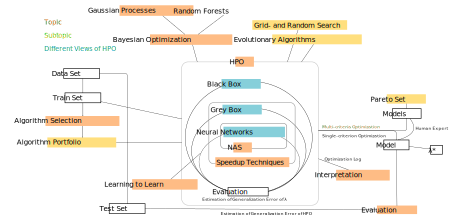
\includegraphics[width = 0.9\linewidth]{images/drawing.pdf}  
    \end{center}
\end{frame}

\begin{frame}{Automate HPO}

  \begin{columns}
    \begin{column}{0.59\textwidth}

      For AutoML the user only supplies \ldots
      \begin{itemize}
        \item dataset
        \item performance measure and
        \item possibly a time limit.
      \end{itemize}

      So far HPO additionally needs \ldots
      \begin{itemize}
        \item one learning algorithm (to generate Inducer $\inducer$),
        \item search space $\pcs$ to chose $\conf$ from,
        \item a resampling strategy to evaluate $\cost(\conf)$ and
        \item optimization algorithm.
      \end{itemize}

      To build an AutoML System we have to make these choices automatically.

    \end{column}%
    \begin{column}{0.4\textwidth}
      \begin{center}
        \includegraphics[width = \linewidth]{images/tuning.pdf}    
      \end{center}
    \end{column}
  \end{columns}

\end{frame}

\begin{frame}{Choice of learning algorithm}
  \begin{itemize}
    \item A good AutoML System should consider more than one learning algorithm. More on that later.
    \item A plethora of learning algorithm exists.
    \item Studies\footnote{\href{https://dl.acm.org/doi/10.5555/2627435.2697065}{Delgado et al., JMLR 2014}} and experience have shown that one representative of these categories usually reaches best performance (on tabular data):
    \begin{itemize}
      \item Penalized Regression, SVM, Gradient Boosting, Random Forests, Neural Networks
      \item (tuned) random forests hardly beaten by current AutoML frameworks\footnote{\href{https://arxiv.org/abs/1907.00909}{Gijsbers et al., 2019}}.
      \item Example: Auto-Sklearn 2.0\footnote{\href{https://arxiv.org/abs/2007.04074}{Feurer et al., 2020}} uses: Extra Trees, Gradient Boosting, Passive Aggressive, Random Forest, Linear Model
    \end{itemize}
  \end{itemize}
\end{frame}

\begin{frame}{Choice of Search Space for a Learning Algorithm}
  \begin{columns}
    \begin{column}{0.6\textwidth}
    Which hyperparameters should we consider for a given learning algorithm?
    \begin{itemize}
      \item Ranges often selected based on experience
      \begin{itemize}
        \item Compare to other AutoML Frameworks: e.g.\ Auto-Sklearn 2.0~\lit{\href{https://arxiv.org/abs/2007.04074}{Feurer et al., 2020}} 
      \end{itemize}
      \item Sensitivity analysis does not exist for each learning algorithm
      \item Solution: Analysis of previous HPO runs and learn mapping $\datasets \rightarrow \mathcal{P}(\pcs)$ is risky (leaving out important ranges) and complicated.
      \item Instead: Use big search space $\pcs$ and try to predict good initial design (e.g.\ for Bayesian Optimization).
    \end{itemize}
    \end{column}%
    \begin{column}{0.4\textwidth}
      \begin{center}
        \only<1>{
          \includegraphics[width = 0.8\linewidth]{images/probst2019jmlr_tab1.pdf}
        }
        \only<2>{
          \includegraphics[width = 0.8\linewidth]{images/probst2019jmlr_tab3.pdf}   
        }

        {\tiny Taken from \href{https://www.jmlr.org/papers/volume20/18-444/18-444.pdf}{Probst et al., 2019 JMLR}.}
      \end{center}
    \end{column}
  \end{columns}
\end{frame}

\begin{frame}{Choice of Resampling Strategy}
    \begin{itemize}
      \item Default: 10-fold CV
      \item Huge datasets: Holdout
      \item Tiny datasets: LOO
      \item For class imbalances:
      \begin{itemize}
        \item use stratification.
        \item ensure that validation split includes minority class.
      \end{itemize}
    \end{itemize}
    $\rightarrow$ Create heuristic or let the user decide.
\end{frame}

\begin{frame}{Choice of Optimization Algorithm}
  Choose optimization algorithm based on \ldots
  \begin{itemize}
    \item complexity of search space and
    \item estimated number of possible evaluations
  \end{itemize}

  \begin{itemize}
    \item Complex search space and many possible evaluations $\rightarrow$ Random Search, TPE, BO with RF as Surrogate
    \begin{itemize}
      \item Make use of Grey-Box Optimizers: Hyperband, BOHB
    \end{itemize}
    \item Simple search space and few possible Evaluations $\rightarrow$ BO with Kriging as Surrogate
    \begin{itemize}
      \item Grey-Box: BOHB
    \end{itemize}
    \item Complex search space and few possible evaluations $\rightarrow$ Use good defaults, Meta-Learning
    \item Deep Neural Network Architecture Search $\rightarrow$ NAS Algorithms and possibly HPO on found architecture
  \end{itemize}
\end{frame}



\begin{frame}[containsverbatim,allowframebreaks]{Preprocessing}
  \begin{center}
    \includegraphics[width = 0.5\linewidth]{images/AutoMLPipeline.jpg}  
  \end{center}

  Ideal ML Pipeline steps for AutoML Systems:
  \begin{itemize}
    \item Data Cleaning
    \item Feature Engineering
    \begin{itemize}
      \item Feature Selection
      \item Feature Preprocessing
      \item Feature Construction  
    \end{itemize}
  \end{itemize}

\end{frame}

\begin{frame}{Preprocessing not the strength of Non-commercial AutoML}
  \begin{columns}
    \begin{column}{0.6\textwidth}
      \vspace*{-1cm}
      \begin{center}
        \includegraphics[width = \linewidth]{images/Truong2019Towards_fig2.pdf}
      \end{center}
    \end{column}%
    \begin{column}{0.3\textwidth}
    \small
      Taken from \href{https://doi.org/10.1109/ICTAI.2019.00209}{Truong et al., 2019 ICTAI}.
      \vspace{1em}

      Highlighted: Non-commercial AutoML Frameworks
    \end{column}
  \end{columns}
\end{frame}

\begin{frame}{Cleaning and Feature Selection}
    \begin{columns}
      \begin{column}{0.7\textwidth}

        Data Cleaning can hardly be automatized but a few heuristics exist:
        \begin{itemize}
          \item Remove ID Columns, Columns with mostly unique values
          \item Outlier detection (in the feature space)
          \item Detect time series or spatial data $\rightarrow$ randomized validation might be flawed.
        \end{itemize}

        Feature Selection
        \begin{itemize}
          \item Seldom increases performance but decreases computational costs $\rightarrow$ Multi-criteria optimization.
          \begin{itemize}
            \item Combined Feature Selection and HPO: \lit{\href{https://doi.org/10.1145/3377930.3389815}{Binder et al., 2020 GECCO}}
          \end{itemize}
          \item Happens indirectly in learning algorithm: random forest, lasso regression, \ldots %FIXME More examples.
        \end{itemize}
      \end{column}%
      \begin{column}{0.3\textwidth}
        \begin{center}
          \includegraphics[width = \linewidth]{images/Binder2020multiobjective_fig3.pdf}

          {\tiny Taken from \href{https://doi.org/10.1145/3377930.3389815}{Binder et al., 2020 GECCO}.}
        \end{center}
      \end{column}
    \end{columns}
\end{frame}

\begin{frame}{Preprocessing}
  \begin{itemize}
    \item categorical values:
    \begin{itemize}
      \item Impact Encoding (aka Target Encoding) \\
      \vspace*{-0.5cm}  
        \begin{align*}
          \text{Regression:} \operatorname{Impact}(x) &= \E(\bm{y} | x) - \E(\bm{y}) \\
          \text{Classification:} \operatorname{Impact}(x) &= \operatorname{logit}(P( y = \text{target} | x)) - \operatorname{logit}(P( y = \text{target}))
        \end{align*}
        \vspace*{-0.5cm}  
        \begin{itemize}
          \item Needs regularization (through CV) to prevent target leakage \lit{\href{https://arxiv.org/abs/1611.09477}{Zumel et al., 2019}}
          \item Advantage: Handles unknown categorical levels on test data.
        \end{itemize}
    \end{itemize}
    \item missing values:
    \begin{itemize}
      \item Additional factor column indicating missigness
      \item Replace missing values with out of range or median/mode
      \item Advanced imutation strategies seldomly advantageous (also because data mostly not missing at random)
    \end{itemize}
    \item imbalanced classes:
    \begin{itemize}
      \item over-sampling of minority class
      \item seldomly: under-sampling of majority class
    \end{itemize}
  \end{itemize}
\end{frame}

\begin{frame}{Feature Construction}
  \begin{itemize}
    \item Generic:
    \begin{itemize}
      \item Polynomial Features
      \item Normalization (Box-Cox-Transformation)
      \item PCA
    \end{itemize}
    \item Heuristiscs:
    \begin{itemize}
      \item Detecting Dates, Hours: Transofrm to ``circular'' features within year, month, day, or whatever periodicity we assume \\
      e.g.\ $\tilde x_1 = sin(2\pi \cdot x /24)$ and $\tilde x_2 = cos(2\pi \cdot x /24)$
    \end{itemize}
    \item Combine with external data:
    \begin{itemize}
      \item names $\rightarrow$ gender, ethnicity, age
      \item home adress $\rightarrow$ household income
      \item location + date $\rightarrow$ weather
    \end{itemize}
  \end{itemize}
    
\end{frame}

\begin{frame}{Pipelining}

Most preprocessing steps have parameters or can be switched on/off in the pipeline.

\textbf{Goal:} Find optimal preprocessing parameters $\rightarrow$ HPO

\begin{columns}
  \begin{column}{0.5\textwidth}
  \begin{itemize}
    \item Most prepocessing methods have states similar to the model of an inducer.
    \item Applying preprocessing to the whole dataset leads to overfitting.
    \item Pipeline has to be optimized as a whole: $\pcs = \pcs_{\text{pipeline}} \times \pcs_\inducer$ within the resampling procedure.
  \end{itemize}
  \end{column}%
  \begin{column}{0.5\textwidth}
    \begin{center}
      \includegraphics[page=19, width=\textwidth, trim=20 60 30 35, clip]{images/mlr3Pipelines_graphics}
    \end{center}
  \end{column}
\end{columns}

\end{frame}

\begin{frame}{Optimizing Pipelines}

  \begin{columns}
    \begin{column}{0.5\textwidth}
      \vspace*{-0.5em}
      \begin{itemize}
        \item Introducing different choices for preprocessing
        \item Tuning over multiple learning algorithms
      \end{itemize}
      $\rightarrow$ $\pcs$ becomes hierarchical search space!
      
      \vspace*{0.5em}

      Suitable optimizers:
      \begin{itemize}
        \item Random Search
        \item BO with RF surrogate
        \item Evolutionary approaches (similar to NAS)
      \end{itemize}

      Possible improvements:
      \begin{itemize}
        \item Instead of only keeping best setting: build ensemble of good configurations (e.g. \lit{\href{https://www.automl.org/wp-content/uploads/2020/07/AutoML_2020_paper_61.pdf}{H2O AutoML, LeDell et al., 2020}})
      \end{itemize}
    \end{column}%
    \begin{column}{0.5\textwidth}
      \begin{center}
        \includegraphics[page=7, width=\textwidth, trim=160 0 30 160, clip]{images/mlr3Pipelines_graphics}
      \end{center}
    \end{column}
  \end{columns}
    
\end{frame}

% \begin{frame}[containsverbatim,allowframebreaks]{Software}

% \begin{itemize}
%   \item DataRobot (comercial, gui)
%   \item H20.ai (comercial but open source, r, python)
%   \item TPOT, Tree-based Pipeline Optimization Tool  (2016-cont, open source, evolutionary approach) % show plot https://github.com/EpistasisLab/tpot
%   \item AutoWEKA (2016, open source)
%   \item mlr3automl (2020, prelim)
%   \item Hyperopt-Sklearn (2014-cont) Only HPO
%   \item Auto-Sklearn (2.0) (2015-cont) BO, ensembles, meta-learning
% \end{itemize}

% \end{frame}



\end{document}
